\section{Muhammad Fahmi (1174021)}

\subsection{Pengertian}
Pengertian geografi adalah bidang ilmu yang secara khusus mempelajari lokasi dan persamaan serta perbedaan spasial dari fenomena fisik, dan manusia di permukaan bumi. \hfill\break
Pendapat lain mengatakan definisi geografi adalah studi tentang karakteristik fisik bumi dan atmosfernya, dan aktivitas manusia yang mempengaruhi dan dipengaruhi, termasuk distribusi populasi dan sumber daya, penggunaan lahan, dan industri. \hfill\break
Secara etimologis, istilah "geografi" berasal dari bahasa Yunani, yaitu kata "geo" yang berarti bumi, dan "graphien" yang berarti pencitraan. Sehingga geografi dapat didefinisikan sebagai ilmu yang menggambarkan segala sesuatu yang ada di permukaan bumi.\hfill\break

Agar lebih memahami apa itu geografi, maka kita dapat merujuk pada pendapat beberapa ahli berikut ini: \hfill\break
\begin{itemize}
	\item Claudius Ptolomaeus
Menurut pendapat Claudius Ptolomaeus, definisi geografi adalah presentasi melalui peta sebagian dan seluruh permukaan bumi.
	\item Preston E. James
Menurut pendapat Preston E. James, definisi geografi adalah ibu dari semua ilmu, ini karena bidang sains selalu berawal dari keadaan bumi yang kemudian beralih ke studi masing-masing ilmu.
	\item Frank Debenham
Frank Debenham mengatakan bahwa pengertian geografi adalah ilmu yang bertugas membuat interpretasi tentang distribusi fakta, menemukan hubungan antara kehidupan manusia dan lingkungan fisik, dan menjelaskan kekuatan interaksi antara manusia dan alam.
	\item Mustofa Bisri
Menurut Mustofa Bisri, definisi geografi adalah ilmu yang menggambarkan permukaan bumi, iklim, populasi, flora dan fauna, serta hasil yang ditemukan di bumi. 
\end{itemize} \hfill\break

\begin{figure}[H]
	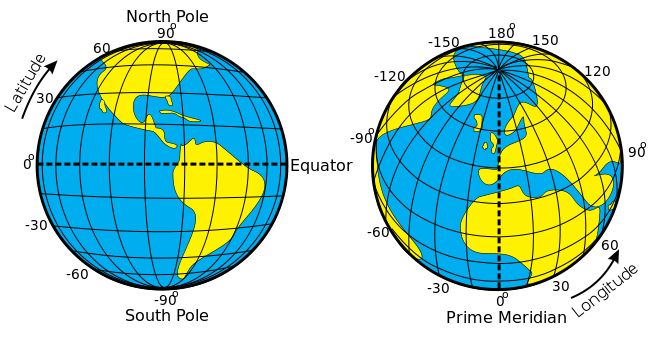
\includegraphics[width=4cm]{figures/1174021/1.png}
	\centering
	\caption{Sistem Informasi Geografis.}
\end{figure}


\subsection{Sejarah}
Sejarah geografi dimulai dengan interaksi antara manusia dan lingkungannya. Ini adalah awal dari perkembangan geografi.
Awalnya, geografi hanya dibahas atau dijelaskan dalam deskripsi umum fakta yang dijelaskan kondisi di bumi. Pada abad ke-18, yaitu era geografi klasik, geografi terbatas pada menjelaskan dan mengumpulkan informasi tentang lingkungan geografis, misalnya: kondisi politik, industri, iklim, terutama di kota-kota besar. Sejarah geografi berlanjut. Lebih tepatnya, pada abad ke-19 geografi mengalami perkembangan dalam sains. Dari apa yang semula hanya dijelaskan, kemudian dikembangkan menjadi lebih spesifik, yaitu dengan menjelaskan lingkungan geografis secara sistematis. \hfill\break

Pada pertengahan abad ke-19, ilmu dalam geografi telah membahas sejauh kondisi yang sebanding, data geografis dan karakteristik antara satu wilayah dan lainnya di bumi. Ini kita kenal sebagai "Geografi Komparatif". Perkembangan geografi tumbuh lebih pesat setelah Perang Dunia Kedua. Yang pada awalnya dikembangkan oleh imigran Amerika dan Inggris yang dikenal sebagai "Geografi Komparatif" kemudian berkembang menjadi "Geografi Global" di mana objek penelitian yang lebih luas meliputi seluruh dunia. Era ini disebut sebagai "era geografi modern". \hfill\break

Geografi Sejarah dari Yunani, Dari pembahasan di atas, kita sudah tahu kapan sejarah geografi dimulai, yaitu sejak interaksi antara manusia dan lingkungannya. Jika demikian, maka esensi sejak Nabi Adam AS turun ke bumi adalah bahwa geografi sudah ada. Tetapi penggalan ilmiah geografi itu sendiri hanya dilakukan untuk pertama kalinya oleh orang Yunani. Dimana dalam perkembangan awal dimotivasi oleh upaya oleh orang-orang Yunani untuk melepaskan diri dari ranah pemikiran dan kepercayaan. Dimana kepercayaan ini meyakini bahwa para dewa ikut campur dalam segala bentuk peristiwa di bumi. \hfill\break

Istilah geografi sebenarnya hanya digunakan pada tahun 1972 ketika sebelumnya menggunakan istilah "ilmu bumi". Istilah ini pertama kali diperkenalkan oleh seorang filsuf dan astronom bernama Eratosthenes (276–194 SM). Kemudian, Claudius Ptoleumaeus meletakkan dasar-dasar ilmu geografis. Sejarah perkembangan geografi terus berlanjut. Immanuel Kant mengembangkan geografi modern dan kemudian Karl Ritter juga mengembangkan geografi sosial. \hfill\break

Nah, sekarang kita membahas sejarah SISTEM INFORMASI GEOGRAFIS, GIS (Sistem Informasi Geografis) atau Sistem Informasi Geografis adalah sistem informasi yang digunakan untuk memasukkan, menyimpan, memulihkan, mengolah, menganalisis, dan menghasilkan data geografis atau referensi geografis, untuk mendukung memperoleh hasil sesuai dengan perencanaan. Dengan menggunakan GIS akan lebih mudah bagi para pembuat keputusan untuk menganalisis data yang ada. Karena dengan SIG itu juga akan menggambarkan posisi penyebaran data dalam kondisi aktual. \hfill\break

Teknologi Sistem Informasi Geografis dapat digunakan untuk penyelidikan ilmiah, manajemen sumber daya, perencanaan pembangunan, kartografi dan perencanaan rute. Misalnya, GIS dapat membantu perencana untuk menghitung respon darurat dengan cepat jika terjadi bencana alam, atau GIS dapat digunakan untuk mencari lahan basah (lahan basah) yang membutuhkan perlindungan dari perbudakan. \hfill\break

Pengenalan awal GIS tidak lepas dari kemajuan di bidang teknologi, khususnya komputer. Selama perang dunia kedua, data yang benar yang berhasil memperbaiki apa yang diperlukan untuk keperluan militer dalam memprediksi lintasan balistik. Pada awal 1960-an perkembangan dalam ilmu komputer meningkat dan siap digunakan untuk bidang lain di luar militer. Ahli meteorologi, geologi dan geofisika mulai menggunakan komputer dalam pembuatan peta.
Pada tahun 1963 di Kanada muncul CGIS (Sistem Informasi Geografis Kanada), dan kemudian menjadi GIS pertama di dunia. Dua tahun kemudian di Amerika Serikat, sistem yang disebut MIDAS digunakan untuk memproses data sumber daya alam. \hfill\break


\subsection{Koordinat}
Sistem koordinat peta adalah seperangkat aturan yang menentukan koordinat yang ditentukan untuk mewakili titik atau objek pada peta. Aturan ini biasanya mengubah titik asal (origin) yang terkait dengan beberapa titik koordinat untuk mengukur jarak dan sudut untuk menghasilkan koordinat. Sistem koordinat peta yang terkenal di dunia adalah sistem koordinat geografis dan sistem koordinat Universal Transvers Mercator (UTM). \hfill\break

Sistem koordinat geografis atau sering disebut sistem koordinat geodetik dikembangkan oleh Greenwich (dari Inggris) yang mengatur bumi menjadi dua bagian, yaitu irisan melintang yang disebut garis lintang mulai dari garis khatulistiwa (khatulistiwa), membesar ke arah kutub (utara dan selatan) yang terletak membentang dari Greenwich (dekat dengan Inggris) ke barat dan timur. \hfill\break

Sistem koordinat geografis digunakan untuk menentukan titik di Bumi pada garis lintang dan bujur.
Latitude adalah garis horizontal yang mengukur sudut antara titik dan ekuator. Titik di utara khatulistiwa disebut Lintang Utara. Sedangkan titik di selatan khatulistiwa disebut Lintang Selatan. \hfill\break


\subsection {Data Geospasial}
Data geospasial adalah penggambaran lokasi geografis, dimensi atau ukuran / karakteristik objek alami atau buatan manusia yang berada di bawah atau di atas permukaan bumi, data geospasial biasanya disingkat menjadi DG.\hfill\break

Data geospasial dibagi menjadi 2 yaitu:

\begin{enumerate}
	\item Vektor \hfill\break
Vektor adalah salah satu jenis gambar yang dapat dibuat menggunakan corel, adobe illustrator atau dengan aplikasi vektor lainnya. Vektor sering digunakan untuk membuat gambar animasi dan vektor juga digunakan oleh peta goole.
	\item Roshen \hfill\break
Roshen adalah gambar yang diambil dari satelit di luar angkasa, gambar ini adalah tipe jpg, dan pembaruan data gambar ini membutuhkan waktu lama karena prosesnya membutuhkan waktu lama, jenis data ini digunakan oleh Google Earth. 
\end{enumerate}

Data geospasial banyak berguna, baik untuk bisnis maupun untuk pemerintah.
Sebagai contoh, dengan data geospasial kita dapat melihat jalan mana yang padat atau bahkan padat. Dengan mengetahui situasi ini, pihak-pihak yang bernegosiasi seperti polisi lalu lintas dapat menangani seperti mengalihkan arus ke rute alternatif atau memberlakukan jalan satu arah. \hfill\break

\subsection{Link Video}

\begin{figure}[H]
	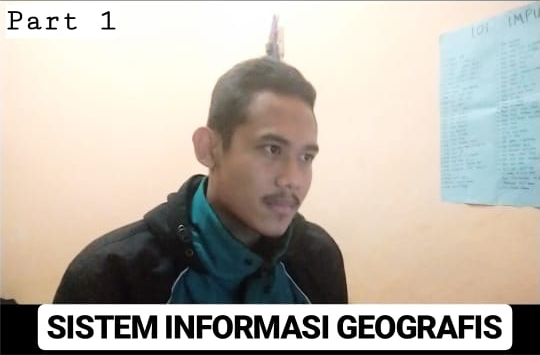
\includegraphics[width=4cm]{figures/1174021/2.png}
	\centering
	\caption{Video.}
\end{figure}

\begin{itemize}
	\item \href{https://www.youtube.com/watch?v=Dw8NGQUF-YQ} {Klik Disini saja !}
\end{itemize}

\subsection{Plagiarism}
\begin{figure}[H]
	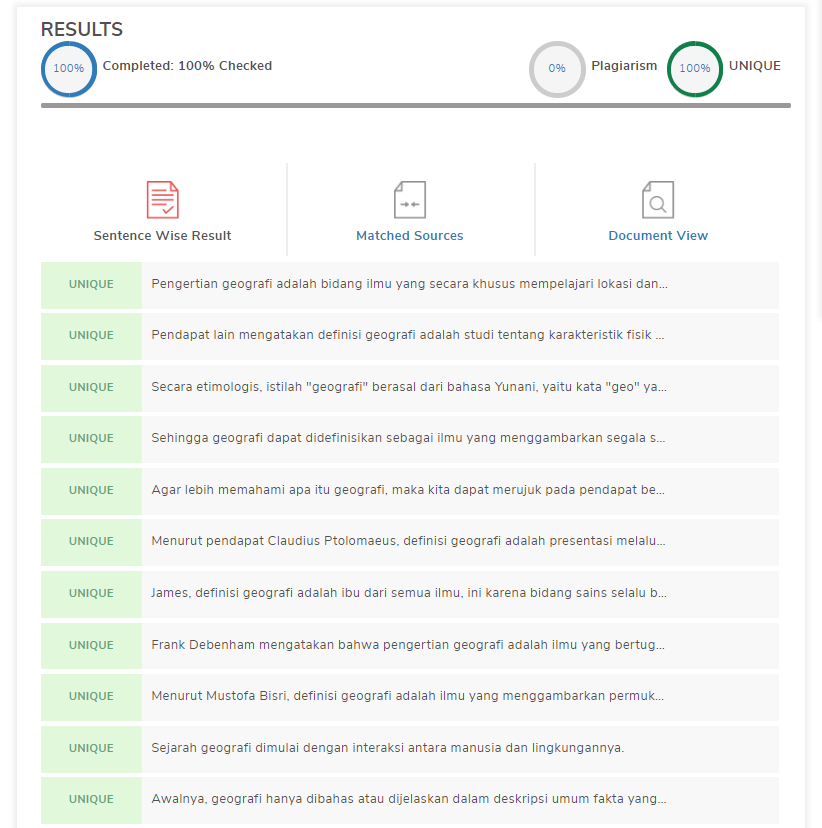
\includegraphics[width=4cm]{figures/1174021/buktiplagi1.png}
	\centering
	\caption{Bukti Tidak Melakukan Plagiat 1}
\end{figure}

\begin{figure}[H]
	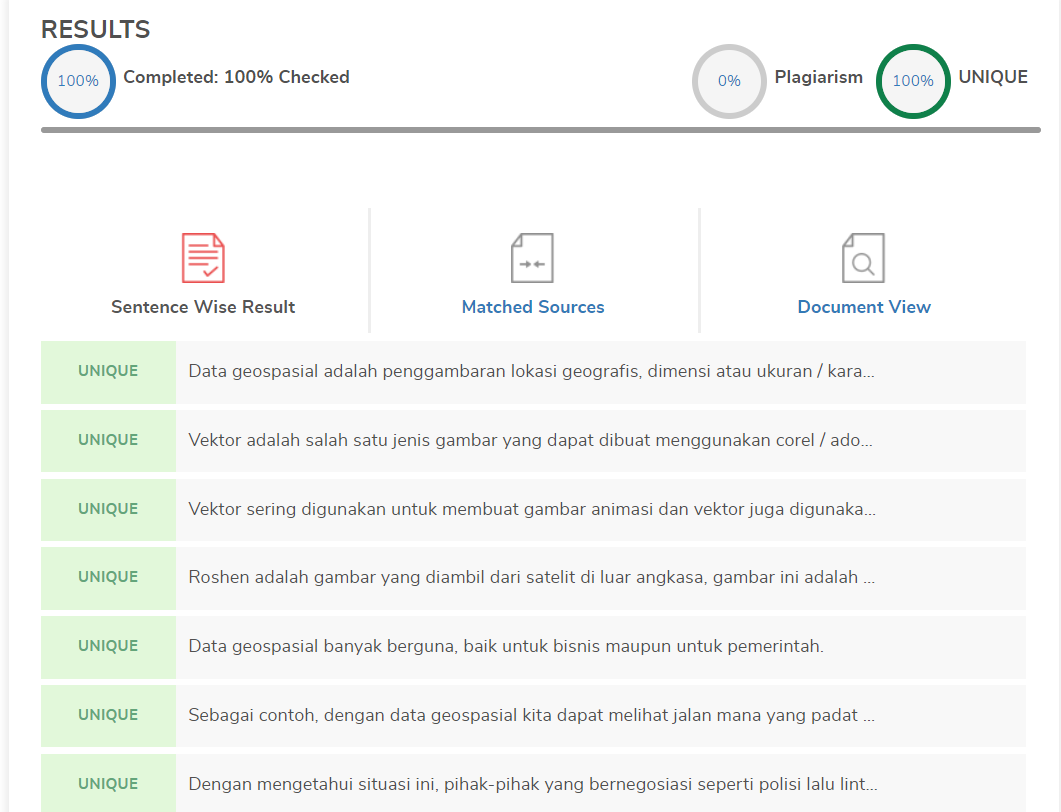
\includegraphics[width=4cm]{figures/1174021/buktiplagi2.png}
	\centering
	\caption{Bukti Tidak Melakukan Plagiat 2}
\end{figure}



